%This is an example for a chapter, additional chapter can be added in the skeleton-thesis
%To generate the final document run latex, build and quick build commands on the skeleton-thesis file not this one.
%This is chapter 2, the default skeleton thesis expects 2 chapters
\chapter{Methodology}
\label{sec:methodology}
%\paragraph{\bfseries Android Over}
%Android is an open source operating system designed for smartphones and other mobile devices whose applications are primarily written in Java, sometimes accompanied by native code, which is then compiled to Dalvik bytecode and run in a virtual machine similar to the Java virtual machine.  Because the quality and trustworthiness of applications varies widely, Android treats all applications as potentially buggy or malicious.  Every application runs as an unpriviledged user with Linux UIDs effectively being used to provide application sandboxes.  To increase code re-usability, the Android application framework forces a componenet-based application model [26].  Instead of having a main() function or any single entry point for execution, Android application of developed in terms of components.

%The applications are composed of four component types:  activity, service, broadcast receiver, and content provider.  Activities are focused windows in which the user interaction takes place; only one activity can be active at a time.  Each activity is a class in the source code and should perform according to events generated by users and the system. Services are designed to run in the background while content providers manage access to data.  Broadcast Receivers are registered with system services and can receive system events, such as re-boot completed, or an SMS received, and so on.  Once a broadcast receiver is registered to receive a system event, the code specified in the broadcast receiver is run whenever the system event is triggered.  Most system events are guarded by permissions, which the applications must declare and get approval for at installation time.

%For automatic exploration, it is neccessary to understand the GUI features in Android.  Each activity corresponds to a screen displayed to the user.  This screen is functionally equivalent to a traditional GUI window, the only difference being that only one screen is shown at a time (with minor exceptions), whereas traditional GUIs can typcally display multiple windows.
%An application's GUI consists of several activities that invoke one another and possibly return results.  At any point in time, only one activity has input focus and processing.  This activity is referred to as the active activity.  When one activity invokes another, the former is paused and the new activity is pushed to the top of the activity stack and made active.  Once an activity has completed its work, it terminates, optionally returning a value, and the next activity on the stack is made active.  Note that activities are not limited to invoking activities within the same application.  A sequence of related activities on the stack is called a task.


%\subsection{Android Overview}   

%Because the quality and trustworthiness of applications varies widely, Android treats all applications as potentially buggy or malicious.  Each application runs in a process with a low-privilege user ID, and applications can access only their own files by default.  Aplications are written in Java (sometimes accompanied by native code), and each application runs in its own Dalvik virtual machine, an optimized Android specific Java VM.  The Android application framework forces a componenet-based application model [26] to increase code reusability.  Applications do not have a main() function or any single entry point for execution but are developed in terms of components.  There are four types of compenents defined in Android's programming model: Activity, Broadcast Receiver, Content Provider and Service. Activity components define an application’s user interface.  Typically, an application developer defines one activity per “screen.” Activities start each other, possibly passing and returning values. Only one activity on the system has keyboard and processing focus at a time; all others are suspended. Service components perform background processing. When an activity needs to perform some operation that must continue after the user interface disappears (such as download a file or play music), it commonly starts a service specifically designed for that action. The developer can also use services as application-specific daemons, possibly starting on boot. Services often define an interface for Remote Procedure Call (RPC) that other system components can use to send commands and retrieve data, as well as register callbacks. Content provider components store and share data using a relational database interface. Each content provider has an associated “authority” describing the content it contains. Other components use the authority name as a handle to perform SQL queries (such as SELECT, INSERT, or DELETE) to read and write content. Although content providers typically store values in database records, data retrieval is implementation-specific—for example, files are also shared through content provider interfaces. Broadcast receiver components act as mailboxes for messages from other applications. Commonly, application code broadcasts messages to an implicit destination. Broadcast receivers thus subscribe to such destinations to receive the messages sent to it. Application code can also address a broadcast receiver explicitly by including the namespace assigned to its containing application.


%Because the quality and trustworthiness of applications varies widely, Android treats all applications as potentially buggy or malicious.  Each application runs in a process with a low-privilege user ID, and applications can access only their own files by default.  Aplications are written in Java (sometimes accompanied by native code), and each application runs in its own Dalvik virtual machine, an optimized Android specific Java VM. The Android operating system limits application privileges through a permission system.  Privileges are requested by the application developer in a manifest which is incorporated into the application package, and approved by the user when the application is installed.  The user may only choose to accept all of the permissions or not install the application -- they can't grant or deny specific permissions.


%Static livraries provide common system and application librariries for applications.  The Android runtime environment is composed of core runtime libraries and the Dalvik virtual machine (VM) - an optimized Android-sepcific Java virtual machine.  Finally the Linux kernel completes the OS and the software stack.  Each Android application runs with a unique user ID, in its own copy of the Dalvik virtual machine, which ensures separation between applications and provides protection.
 
%Android controls access to system resources with installtime permissions categorized into three threat levels : Normal, Dangerous, and Signature/System.  Applications can define their own permissions for purpose of self-protection.  Permissions may be required when interacting with the system API, databases, and the message-passing system.

%This work involves the top three layers.  To test programs running in the Application layer, services from the Application Framework layer and intrumentation tools in the Dalvik VM are used.

%Andorid applications can be composed of four component categores: Activity, Broadcast Receiver, Content Provider and Service.  
%Android defines four component
%types:





%The activity GUI layout is commonly defined in XML but may also be defined programmatically.  As in traditional GUIs, an Android window consists of widgets, which are referred to as views in Android terminology.  The Android library supplies several useful views which may either be standalone (e.g., buttons) or act as containers for other views.  In addition to the window layout, an activity can define a menu that appears when the user presses the physical "Menu" button on the phone.

%Applications run at the very top of the platform with their Services, such as the Acitivity Manager , which controls the activities for each application and Content Providers, which load the content provider defined by each application while restricting data accessibility across applications, located in the Application Framework layer


\toolname, a system for evaluating how removing permissions impacts the behavior of Android applications, was designed for the purpose of this study and leverages the Android emulator, APKTool, and AndroidViewClient.  To evaluate each application, \toolname\ automatically runs the application, supplies it with various UI events, detects when the application crashes, and logs the cause of the crash.  \toolname\ consists of the following components (see Figure~\ref{fig:diagram}).

%\FloatBarrier
\begin{figure*}[b]
\figsp
\centerline{\resizebox{0.9\linewidth}{!}{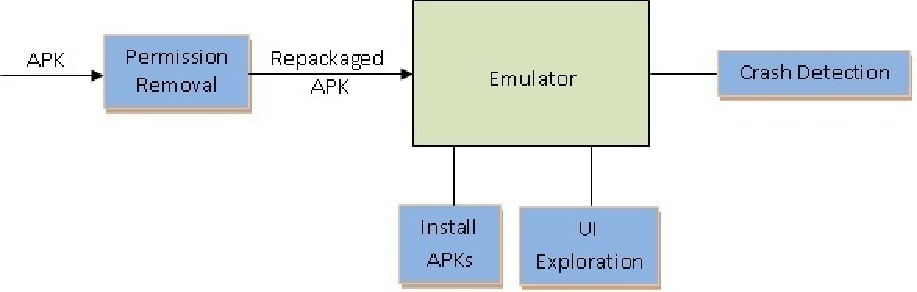
\includegraphics{flowchart}}}
\caption{PyAndrazzi Component Diagram}
\label{fig:diagram}
\end{figure*}
%\FloatBarrier

%\FloatBarrier
\begin{figure*}[b]
\centerline{\resizebox{0.5\linewidth}{!}{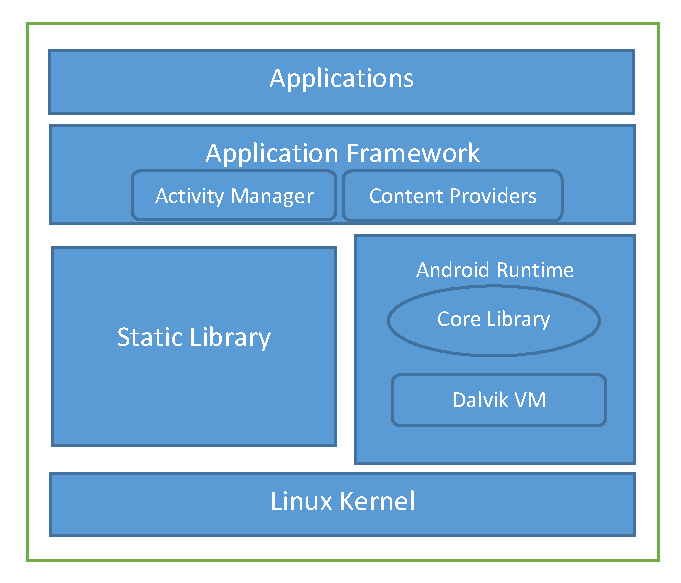
\includegraphics{android_architecture}}}
\caption{Android Platform Architecture}
\label{fig:architecture}
\end{figure*}
%\FloatBarrier

\paragraph{\bfseries Android Emulator}
The Android platform is comprised of 4 layers: Applications, an Application Framework layer, a Library/VM layer, and, the Linux Kernel (see Figure \ref{fig:architecture}).  Applications run at the very top of the platform with their Services, such as the Acitivity Manager and Content Providers, located in the Application Framework layer.  The Library/VM layer contains static libraries and the Android runtime environment.  An Android emulator is an application that provides a virtual mobile device on which Android applications can be run.  It runs a full Android system stack, down to the kernel level, that includes a set of pre-installed applications, such as the dialer, that applications can access.  The emulator provides dynamic binary translation of device machine code to the OS and processor architecture of the development machine.  The configuration of AVDs(Android Virtual Devices), allows for the specification of the Android platform (i.e. API 17) to run in the emulator, the set of hardware options and the emulator skin.  The Android system images, available through the Android SDK Manager, contain code for the Android Linux kernel, the native libraries, the Dalvik VM, and the various Android packages (such as the Android framework and preinstalled applications).  



The Android SDK Manager provides system images for both x86 and arm architectures, however, the x86 image does not include the map libraries.  To improve performance, \toolname~employs the x86 architecture and kvm acceleration, and utilizes a modified x86 system image that includes the missing libraries.  When launching an emulator, the desired AVD configuration is specified.  Each AVD functions as an independent device, with its own private storage for user data, SD card, etc. 

%When launchincg the emulator with an AVD configuration, it automatically loads the user data and SD card data from the AVD directory. By default, the emulator stores the user data, SD card data, and cache in the AVD directory.



\paragraph{\bfseries Permission Removal}
APKTool is an opensource tool developed for reverse engineering closed, binary Android applications. It decompiles bytecode to smali, an assembly language for the dex format used by Android's Davlik VM, and is able to re-build applications after modifications are made.  \toolname\ uses APKTool to decode the application's APK file.  Then, it removes the permission being evaluated from the applications AndroidManifest.xml file and collects the Activity names for use in automated testing.  Finally, it rebuilds the APK and signs it using Android's built-in debug key.



\paragraph{\bfseries Installation and Execution}
\toolname\ installs and runs applications in emulators.  It utilizes the standard android debug bridge(ADB) to install and uninstall applications and, due to its increased stability, uses the android debug bridge(ADB) developed by ~\cite{Milano} to provide UI inputs to applications.

%For automatic exploration, it is neccessary to understand the GUI features in Android.  Each activity corresponds to a screen displayed to the user.  This screen is functionally equivalent to a traditional GUI window, the only difference being that only one screen is shown at a time (with minor exceptions), whereas traditional GUIs can typcally display multiple windows.
%An application's GUI consists of several activities that invoke one another and possibly return results.  At any point in time, only one activity has input focus and processing.  This activity is referred to as the active activity.  When one activity invokes another, the former is paused and the new activity is pushed to the top of the activity stack and made active.  Once an activity has completed its work, it terminates, optionally returning a value, and the next activity on the stack is made active.  Note that activities are not limited to invoking activities within the same application.  A sequence of related activities on the stack is called a task.

\paragraph{\bfseries Automatic UI Exploration}
\toolname\ needs to execute as much code as possible to maximize the number of adverse effects resulting from permission removal.  Thus, to maximize coverage, \toolname\ takes the list of Activities for each application and executes each one starting with the \texttt{Main} Activity.  During each Activity, \toolname\ performs a series of pseudo-random screen touches.  This functionality is implemented using a UI introspection approach based on the AndroidViewClient library~\cite{Milano}.  Using this method, \toolname\ is able to query the screen for click-able elements and perform "random" touches with a high probability of changing the application state.      

\paragraph{\bfseries Crash Detection}
\toolname\ communicates with the emulator's ActivityManager monitor to watch for and acquire data on all crash events and their associated package and activity names.  When an application crashes due to a fatal error, such as a \texttt{SecurityException}, a separate thread communicating with the emulator's ActivityManager, will notify the testing thread, which will record the cause of the crash and launch the next Activity.  A similar sequence occurs when a touch results in leaving an application; the thread communicating with Android's ActivityManager, detects that the application is no longer running in the foreground and notifies the testing thread, which then touches the back button.  This ensures the exceptions generated are from the specific application in question.